\chapter{Distribuição de Chaves}
\label{cha:distribuicao-chaves}

Todos os sistemas criptográficos que vimos até aqui são simétricos, ou seja, eles assumem que as partes compartilham um dado sigiloso que chamamos de {\em chave}.
Discutimos como gerar chaves, mas não tratamos ainda de um problema central da criptograia: como distribuir as chaves.
Nesta seção veremos dois modelos bastantes distintos, o primeiro pressupõe a existência de uma autoridade central capaz de assumir a tarefa, o segundo inaugura um novo paradigma de critpografia chamado {\em criptografia assimétrica} que será mais extensamente discutido nos próximos dois capítulos.

\section{Centro de Distribuição de Chaves}
\label{sec:kdc}

No modelo de Centro de Distribuição de Chaves (KDC), cada usuário possui uma {\em chave permanente}.
Essas chaves são gerenciadas por um administrador que centraliza a responsabilidade sobre a distribuição de chaves.
As chaves são criadas pelo administrador que as entrega pessoalmente para cada usuário verificando sua identidade.
Quando Alice quer se comunicar com Bob os seguintes passos são seguidos:

\begin{enumerate}
\item Alice faz uma requisição para o administrador de que pretende falar com Bob.
\item O administrador gera uma chave efêmera $k$ para a comunicação e envia duas cópias para Alice, uma criptografada pela chave permanente de Alice $E(k_A, k)$ e uma criptografada com a chave permanente de Bob $E(k_B, k)$.
\item Alice então encaminha $E(k_B, k)$ para Bob.
\end{enumerate}

\begin{center}
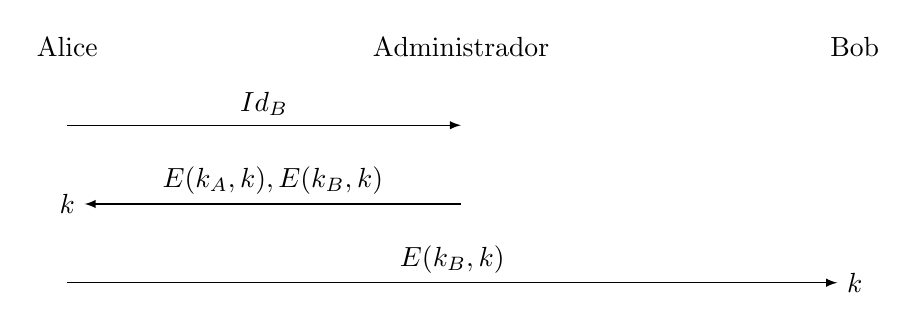
\begin{tikzpicture}[node distance=2cm,auto,>=latex]
\node (alice) at (0, 2){Alice};
\node (bob) at (10, 2) {Bob};
\node (servidor) at (5, 2) {Administrador};

\node (k1) at (0,0) {$k$};
\node (k2) at (10,-1) {$k$};

\path[->] (0,1) edge node[above]{$Id_B$} (5,1);
\path[->] (5,0) edge node[above]{$E(k_A,k), E(k_B,k)$} (k1);
\path[->] (0,-1) edge node[above]{$E(k_B,k)$} (k2);
\end{tikzpicture}
\end{center}

Depois da conversa Alice deve descartar a chave efêmera e eventualmente pedir uma nova para o administrador quando precisar voltar a se comunicar com Bob.

Uma implementação bastante popular do modelo KDC é o protocolo Kerberos\footnote{Uma apresentação compreensível do protocolo está disponível no livro de Paar e Pelzl \cite{Paar09} ou em uma aula gravada e disponível em: https://www.youtube.com/watch?v=iaH8UG2yMg4}.

Além de pressupor a existência de um administrador confiável que gerencie todas as chaves permanentes, os modelo baseados em KDC possuem o que chamamos de {\em ponto único de falha}.
Se o servidor do administrador sair do ar, por exemplo, todas as comunicações seguras ficarão impedidas.
Ou seja, mesmo em um ambiente fechado e com hierarquia estabelecida, esse modelo não é ideal, em um ambiente aberto ele é totalmente inadequado.

\section{Protocolo de Diffie-Hellman}
\label{sec:diffie-hellman}

Em um ambiente aberto não é realista imaginar que as partes podem encontrar o administrador de antemão.
Surpreendentemente existem formas de trocar chaves que podem ser feitas diretamente pelas partes por meio de um canal inseguro.
O esquema que mostraremos nesta seção é conhecido como {\em protocolo de Diffie-Hellman} e inaugura o paradigma revolucionário da {\em criptografia assimétrica} que veremos nos próximos capítulos \cite{Diffie76}.
Informalmente, o protocolo funciona da seguinte forma: Alice envia um dado público para Bob e vice-versa, ao fim do processo ambas as partes são capazes de gerar um mesmo valor que pode ser usado em um KDF para gerar uma chave, porém, para um observador (Eva) que só teve acesso aos dados públicos, isso não é possível.
Para explicar o protocolo precisamos definir o que são grupos, geradores e grupos cíclicos e precisamos apresentar o {\em problema do logaritmo discreto} cuja dificuldade é condição necessária -- apesar de insuficiente -- para a segurança do protocolo.

Um {\em grupo} é uma estrutura algébrica $\mathbb{G} = \langle G, \circ \rangle$ em que $G$ é um conjunto e $\circ$ uma operação binária que satisfaz as seguintes propriedades:
\begin{itemize}
\item[] {\bf (fecho)} Se $f, g \in G$ então $f \circ g \in G$.
\item[] {\bf (identidade)} Existe um elemento $1 \in G$ tal que $1 \circ f = f \circ 1 = f$ para todo $f \in G$.
\item[] {\bf (inverso)} Para todo $g \in G$ existe $h \in G$ tal que $g \circ h = 1$ (é possível mostrar que $h$ é único para cada $g$ e, portanto, o denotaremos $g^{-1}$).
\item[] {\bf (associatividade)} Para todo $f,g,h \in G$ temos que $(f \circ g) \circ h = f \circ (g \circ h)$.
\end{itemize}

Um grupo é dito {\em finito} se $G$ é finito, neste caso, $|G|$ é a {\em ordem} do grupo.
Um grupo é {\em abeliano} se satisfaz o seguinte:
\begin{itemize}
\item[] {\bf (comutatividade)} Para todo $f, g \in G$ temos que $f \circ g = g \circ f$.
\end{itemize}

Diversas estruturas familiares como $\langle \mathbb{Z}, + \rangle$ e $\langle \mathbb{Q}^\star, \cdot \rangle$ são grupos abelianos, mas não são finitos.
No próximo capítulo demonstraremos que certas estruturas são grupos finitos.
Por ora vamos apenas apresentar um grupo finito como exemplo sem uma demonstração para esse fato:
\begin{example}
  A estrutura $\langle \mathbb{Z}_p^\star, \cdot \rangle$ em que $p$ é primo, $\mathbb{Z}_p^\star = \{1, 2, \dots, p - 1 \}$ e a operação de multiplicação é calculada módulo $p$ é um grupo.
  \begin{multicols}{2}
    \begin{itemize}
      \item[] $1^{-1} \equiv 1\ mod\ 7$
      \item[] $2^{-1} \equiv 4\ mod\ 7$
      \item[] $3^{-1} \equiv 5\ mod\ 7$
    \end{itemize}
    \begin{itemize}
      \item[] $4^{-1} \equiv 2\ mod\ 7$
      \item[] $5^{-1} \equiv 3\ mod\ 7$
      \item[] $6^{-1} \equiv 6\ mod\ 7$
    \end{itemize}
  \end{multicols}
\end{example}

Nos será útil expressar a operação de {\em exponenciação} de um elemento do grupo $g \in G$ em relação a um inteiro positivo $m$:
\begin{displaymath}
  g^m := \underbrace{g \circ \dots \circ g}_m
\end{displaymath}


\begin{theorem}
\label{theo:gen-euler}
  Seja $\mathbb{G} = \langle G, \circ \rangle$ um grupo abeliano finito e $m = |G|$, então para qualquer $g \in G$ temos que $g^m = 1$.
\end{theorem}
\begin{proof}
  Note que se $g \circ g_i = g \circ g_j$ então $g_i = g_j$ (basta multiplicar ambos os lados por $g^{-1}$).
  Assim temos que $\{(g \circ g_1), \dots, (g \circ g_m)\} = G$, porque todos os elementos do conjunto da esquerda são elementos de $G$ e são distintos.
  O seja:

  \begin{eqnarray*}
    g_1 \circ \dots \circ g_m & = & (g \circ g_1) \circ \dots \circ (g \circ g_m)\\
                              & = & g^m \circ (g_1 \circ \dots \circ g_m)
  \end{eqnarray*}
  Multiplicando ambos os lados pelo inverso de $g_1 \circ \dots \circ g_m$ temos que $g^m = 1$.
\end{proof}

Se $\mathbb{G} = \langle G, \circ \rangle$ é um grupo finito e $g \in G$ então definimos o conjunto dos elementos {\em gerados} por $g$ da seguinte forma:

\begin{displaymath}
  \langle g \rangle := \{g^0, g^1, \dots \}
\end{displaymath}

A {\em ordem} de um elemento $g \in G$ é o menor $i$ tal que $g^i = 1$.
Pelo teorema anterior temos que $i \leq |G|$ e, portanto, se $G$ é finito, $\langle g \rangle$ é sempre finito.
Um grupo é chamado de {\em cíclico} se existe um elemento $g$, chamado de {\em gerador} cuja ordem é $|G|$.
Ou seja, em um grupo cíclico temos que $\langle g \rangle = G$ para algum $g$.

Se $\mathbb{G}$ é um grupo cíclico e $g$ é um gerador então para qualquer $h \in G$ existe um inteiro $x$ tal que $g^x = h$.
Dizemos que $x$ é o {\em logaritmo} de $h$ na base $g$.


\begin{example}
Considere o grupo $\langle \mathbb{Z}_7^\star, \cdot \rangle$:
\begin{itemize}
\item $\langle 2 \rangle = \{1, 2, 4\}$. A ordem de $2$ é $3$ e, portanto, $2$ não é um gerador de $\mathbb{Z}_7^\star$.
Além disso, neste grupo $log_2(1) = 0$, $log_2(2) = 1$ e $log_2(4) = 2$.
\item $\langle 3 \rangle = \{1, 3, 2, 6, 4, 5\}$. A ordem de $3$ é $6$, portanto $3$ é um gerador de $\mathbb{Z}_7^\star$ e o grupo é cíclico.
Além disso, neste grupo $log_3(1) = 0$, $log_3(2) = 2$ e $log_3(3) = 1$, $log_3(4)= 4$, $log_3(5) = 5$ e $log_3(6) = 3$.
\end{itemize}
\end{example}


O {\em protocolo de Diffie-Hellman} que funciona da seguinte maneira:
\begin{enumerate}
\item Alice roda $\mathcal{G}(1^n)$ para gerar um grupo cíclico $\mathbb{G}$ e um gerador $g$
\item Alice sorteia $x \leftarrow \mathbb{Z}_n$ e computa $h_A = g^x$ usando o algoritmo eficiente de exponenciação
\item Alice envia $\mathbb{G}$, $g$ e $h_A$ para Bob
\item Bob sorteia $y \leftarrow \mathbb{Z}_n$, computa $h_B = g^y$ e envia para Alice.
\item Ao fim do processo Alice computa $h_B^x = (g^y)^x = g^{xy}$ e Bob computa $h_A^y = (g^x)^y = g^{xy}$.
\end{enumerate}

Ao fim do procedimento tanto Alice, quanto Bob são capazes de produzir $g^{xy}$, a primeira porque possui $x$ e $g^y$ e o segundo porque possui $y$ e $g^x$.
Quem observa a comunicação, porém, só possui $g^x$ e $g^y$.
Caso esse observador seja capaz de calcular o $log_g(g^x) = x$ então ele seria capaz de quebrar o protocolo.
O ataque força bruta neste caso seria testar todos os valores possíveis de $x$ até encontar o correto.
Este ataque é linear no valor de $x$, mas é exponencial no tamanho de $x$ (note que para escrever o número $x$ em notação binária usamos espaço proporcional a $log_2(x)$).

Porém, quando Bob calcula $(g^{y})^x$ ele pode usar um algoritmo muito mais eficiente, um que é linear no tamanho de $x$.
A maneira ingênua de calcular a exponenciação se baseia no seguinte invariante:
\begin{displaymath}
  g^m = g^{m-1} \circ g
\end{displaymath}
Com isso reduzimos o problema a um problema um pouco mais simples e paramos quando $m = 0$, pois neste caso $g^0 = 1$.
Essa constatação dá origem ao seguinte algoritmo:

\begin{codebox}
\Procname{$\proc{Exp}(g, m)$}
\li \Comment Recebe $g \in \mathbb{G}$ e $m \in \mathbb{N}$
\li \Comment Devolve $g^m$
\li \If $m = 0 $
\li \Then \Return $1$
\End
\li \Return $\proc{Exp}(g, m-1) \circ g$
\End
\end{codebox}

Podemos estimar o tempo de $\proc{Exp}$ resolvendo a seguinte recorrência:

\begin{eqnarray*}
  T(m) & = & T(m - 1) + \Theta(1)\\
  T(1) & = & \Theta(1)
\end{eqnarray*}

Não é difícil mostrar que $T(m) = \Theta(m)$.
Ou seja, esse algoritmo é linear em relação a $m$ e exponencial em relação ao tamanho de $m$.

Podemos fazer bem melhor do que isso usando o seguinte invariante:
\begin{displaymath}
  g^m = \left\{
    \begin{array}{lcl}
      g^{\lfloor \frac{m}{2} \rfloor} \circ  g^{\lfloor \frac{m}{2} \rfloor} & \textrm{se} & m \textrm{ é par}\\
      g^{\lfloor \frac{m}{2} \rfloor} \circ  g^{\lfloor \frac{m}{2} \rfloor} \circ g & \textrm{se} & m \textrm{ é ímpar}\\
    \end{array}
    \right.
\end{displaymath}

Esse invariante produz o seguinte algoritmo:
\begin{codebox}
\Procname{$\proc{FastExp}(g, m)$}
\li \Comment Recebe $g \in \mathbb{G}$ e $m \in \mathbb{N}$
\li \Comment Devolve $g^m$
\li \If $m = 0 $
\li \Then \Return $1$
\End
\li $x \gets \proc{FastExp}(g, \lfloor \frac{m}{2} \rfloor)$
\li \If $m$ é par
\li \Then \Return $x \circ x$
\li \Else \Return $x \circ x \circ g$
\End
\end{codebox}


Estimamos o tempo de $\proc{FastExp}$ resolvendo a seguinte recorrência:

\begin{eqnarray*}
  T(m) & = & T(\lfloor \frac{m}{2} \rfloor) + \Theta(1)\\
  T(1) & = & \Theta(1)
\end{eqnarray*}

Vimos no curso de Introdução à Análise de Algoritmos que $T(m) = \Theta(log_2(m))$.
Em outras palavras, o problema da exponenciação pode ser resolvido lineramente no tamanho da entrada.

\begin{example}
  Simularemos a execução de $\proc{FastExp}(2, 10)$ em $\langle \mathbb{Q}, \cdot \rangle$.
\begin{displaymath}
  \begin{array}{ll}
    FastExp(2, 10) = x \cdot x = 2^{10} & x = FastExp(2, 5) = 2^5 \\
    FastExp(2, 5)  = x \cdot x \cdot 2 = 2^5 & x = FastExp(2, 2) = 2^2\\
    FastExp(2, 2)  = x \cdot x = 2^2 & x = FastExp(2, 1) = 2\\
    FastExp(2, 1)  = x \cdot x \cdot 2 = 2 & x = FastExp(2, 0) = 1\\
    FastExp(2, 0)  = 1 \\
  \end{array}
\end{displaymath}
\end{example}

O {\em problema do logaritmo discreto} pode ser descrito pelo seguinte jogo:
\begin{enumerate}
\item O sistema recebe o parâmetro de segurança $1^n$ e usa $\mathcal{G}$ para gerar um grupo cíclico $\mathbb{G} = \langle G, \circ \rangle$ com gerador $g$ e ordem $n$
\item O sistema escolhe $h \leftarrow G$ e manda para o adversário $\mathbb{G}$, $g$ e $h$.
\item O adversário produz $x \in \mathbb{Z}_n$
\end{enumerate}

O desafio do adversário é produzir $x$ tal que $g^x = h$.
Ou seja:
\begin{displaymath}
  DLog_{\mathcal{A}, \mathcal{G}}(n) = \left\{
    \begin{array}{lcl}
      1 & \textrm{se} & g^x = h\\
      0 & \textrm{c.c.} &\\
    \end{array}
    \right.
\end{displaymath}

Dizemos que o {\em problema do logaritmo discreto é difícil} se para todo adversário eficiente $\mathcal{A}$ existe uma função desprezível $\varepsilon$ tal que:
\begin{displaymath}
  Pr[DLog_{\mathcal{A}, \mathcal{G}}(n) = 1] \leq \varepsilon(n)
\end{displaymath}

A dificuldade do problema do logaritmo discreto é condição necessária, porém insuficiente, para a segurança do protocolo de Diffie-Hellman.
Algumas estruturas matemáticas são adequadas para produzir grupos cíclicos cujo problema do logaritmo discreto é considerado difícil.
Duas muito usadas na prática são os {\em resíduos quadráticos de grupos de tamanho primo} e as {\em curvas elípticas} (Apêndice \ref{cha:ciclicos}).

Caso o problema do logaritmo discreto não seja difícil, Eva seria capaz de produzir $x$ e $y$ a partir de $g^x$ e $g^y$ e descobrir o valor de $g^{xy}$.
Se o sistema for seguro, porém, o melhor que Eva pode fazer é tentar todos os valores de $\mathbb{Z}_n$ até encontrar $x$ ou $y$.
Escolhendo grupos de ordem suficientemente grande, essa tarefa é computacionalmente inviável.
Uma vez que as partes possuem o mesmo valor secreto, elas podem utilizá-lo para alimentar um KDF e gerar chaves para um sistema de criptografia simétrico.

No modelo, assumimos que o grupo e o gerador são criados sempre que as partes decidem se comunicar.
Na prática o mais comum é que esses parâmetros sejam definidos pelo protocolo e reutilizados em todas as comunicações.
Isso não deve afetar de nenhuma forma na segurança do sistema.

O protocolo de Diffie-Hellman permite às partes compartilharem uma chave secreta sem a necessidade de se encontrarem pessoalmente, ou de confiarem em alguma autoridade que as encontrou separadamente.
Note que o protocolo não garante que as partes saibam se a chave que receberam foi de fato enviada por quem eles imaginam que as enviou.
No Capítulo \ref{cha:assinaturas-digitais} voltaremos a este problema chamado de {\em ataque Man In The Middle}.

\section{Exercícios}
%\label{sec:exercicios}

\begin{exercicio}
  Mostre que se $n|a$ e $n|b$ então para quaisquer $r$ e $s$ temos que $n|(a \cdot r + b \cdot s)$.
\end{exercicio}

\begin{exercicio}
\label{ex:grupo}
  Considere a estrutura $\langle \mathbb{Z}_{12}, \cdot \rangle$ em que a multiplicação é calculada módulo 12.
Mostre que $6$ não possui inverso nesta estrutura e, portanto, ela não é um grupo.
\end{exercicio}

\begin{exercicio}
  Considere as estruturas $\langle \mathbb{Z}_n, + \rangle$ formadas pelo conjunto $\mathbb{Z}_n := \{0, \dots, n-1\}$ e a operação de soma ($+$) módulo $n$.
  Mostre essa estrutura é um grupo cíclico para qualquer valor de $n \geq 1$ e que o número $1$ é sempre um gerador nesses grupos. (Dica: Você precisa mostrar que a operação satisfaz fecho, associatividade, possui elemento neutro e inverso. Depois você deve mostrar que o elemento $1$ gera todos os elementos do grupo.)

  Por que o grupo $\langle \mathbb{Z}_n, +\rangle$ não é um bom candidato para ser usado no protocolo de Diffie-Hellmann.
\end{exercicio}

\begin{exercicio}
  Descreva um ataque força-bruta contra o protocolo de Diffie-Hellman.
  Em termos assintóticos em relação ao tamanho da entrada, qual é o consumo de tempo deste ataque?
\end{exercicio}
